\documentclass[12pt, letterpaper]{article}

\usepackage[margin=1in]{geometry}
\usepackage{mathptmx}
\usepackage[T1]{fontenc}
\usepackage{setspace}
\usepackage{graphicx}
\usepackage{booktabs}
\usepackage{array}
\usepackage{siunitx}
\usepackage{hyperref}
\usepackage{amsmath}
\usepackage{caption}
\usepackage{float}

\singlespacing
\sisetup{group-separator = {,}, group-minimum-digits = 4}

\hypersetup{
  colorlinks=true,
  linkcolor=black,
  citecolor=black,
  urlcolor=blue
}

\title{Section II --- Case III: Defined Contribution Plan and MPF Retirement Planning}
\author{AMA1D03 Introduction to Pension Mathematics}
\date{}

\begin{document}

\begin{titlepage}
  \centering
  \vspace*{2cm}
  {\LARGE\bfseries Section II --- Case III:\\[0.4em]
  Defined Contribution Plan and MPF Retirement Planning\par}
  \vspace{1.5cm}
  {\large AMA1D03 Introduction to Pension Mathematics\par}
  \vfill
  {\large \today\par}
\end{titlepage}
\setcounter{page}{1}

\section*{(a) Descriptions of the Defined Contribution Plan and Its Application in the Pension System}

\subsection*{1. Defined Contribution (DC) versus Defined Benefit (DB)}

Under a \textbf{defined contribution (DC)} plan, the \textbf{contribution side is fixed but the benefit is uncertain}. The employer and/or employee contribute a specified amount into an individual account; the terminal value depends on contributions, investment returns, and fees. Investment and longevity risks are borne primarily by the member.

By contrast, a \textbf{defined benefit (DB)} plan has a \textbf{fixed benefit formula but uncertain required contributions}. The sponsor uses actuarial assumptions to set funding levels and bears most investment and longevity risk if the plan is underfunded. Hong Kong's Occupational Retirement Schemes (ORSO) may be structured as either DC or DB, operating alongside mandatory MPF as part of the second pillar.

Hong Kong's Mandatory Provident Fund (MPF) System, launched on \textbf{1 December 2000}, is a compulsory DC scheme. It forms the \textbf{second pillar} of Hong Kong's retirement protection framework:
\begin{itemize}
  \item \textbf{First pillar:} Flat-rate, means-tested cash benefits---CSSA (last-resort safety net), Old Age Living Allowance (OALA, for lower-income seniors), and Old Age Allowance (OAA, broader but smaller)
  \item \textbf{Second pillar:} MPF mandatory and voluntary contributions (plus ORSO where applicable)
  \item \textbf{Third pillar:} Personal savings, insurance, and family support
\end{itemize}

Hong Kong has \textbf{no earnings-related public pension}. First-pillar benefits are fixed amounts, so MPF is the core retirement base for the middle class---a structural difference from Canada (CPP) or the US (Social Security).

\subsection*{2. Types of MPF Schemes}

According to the Mandatory Provident Fund Schemes Authority (MPFA), MPF schemes are classified into three main types:

\begin{table}[H]
  \centering
  \caption{Types of MPF schemes}
  \begin{tabular}{@{}p{3.2cm}p{9.8cm}@{}}
    \toprule
    Scheme Type & Description \\
    \midrule
    Master Trust Schemes & Open to employees of participating employers and self-employed persons \\
    Employer-sponsored Schemes & Only for employees of a single employer \\
    Industry Schemes & For employees in specific industries (e.g., catering, construction) \\
    \bottomrule
  \end{tabular}
\end{table}

Each employee has a personal account within a scheme. When changing jobs, accrued benefits are portable and can be transferred to the new employer's scheme or retained in a personal account.

\subsection*{3. Mandatory and Voluntary Contributions}

\textbf{Mandatory Contributions (MC):}
\begin{itemize}
  \item Employee and employer each contribute \textbf{5\%} of relevant income
  \item Relevant income is subject to minimum (HK\$7,100) and maximum (HK\$30,000) monthly thresholds
  \item If monthly income is below HK\$7,100, the employee makes no mandatory contribution, but the employer still contributes 5\% of HK\$7,100
  \item Maximum mandatory contribution per party: HK\$1,500 per month
\end{itemize}

\textbf{Voluntary Contributions:}
\begin{itemize}
  \item \textbf{In-scheme voluntary contributions (VC):} extra contributions within an MPF scheme; no salaries-tax deduction; withdrawal rules follow mandatory contributions
  \item \textbf{Tax Deductible Voluntary Contributions (TVC):} separate personal accounts; up to \textbf{HK\$60,000 per year} deductible for salaries tax; more flexible withdrawal conditions
\end{itemize}

In Case III, Peter and Mary each contribute HK\$1,000 (5\% of HK\$20,000 salary), matched equally by their employers, giving a total monthly contribution of \textbf{HK\$2,000}.

\subsection*{4. Benefits, Withdrawal, and Retirement Age}

Members can generally withdraw accrued benefits when reaching age \textbf{65}. Other withdrawal conditions include permanent departure from Hong Kong, total incapacity, terminal illness, early retirement at age 60 with cessation of employment, \textbf{small-balance withdrawal} (total accrued benefits not exceeding HK\$5,000), and \textbf{death benefits} payable to nominated beneficiaries.

Upon withdrawal, members may take a lump sum or convert part of the balance into an annuity through the MPF platform. Annuities are the primary tool for hedging \textbf{longevity risk}---the key vulnerability of DC plans where members outlive their account balances.

\subsection*{5. Investment Options, Returns, and Fees}

MPF offers multiple fund types: Hong Kong, China, Asia, and global equity funds; mixed assets; bond and guaranteed funds; and index-tracking funds such as the Tracker Fund of Hong Kong.

Members bear \textbf{investment risk}. Fund managers charge management fees, typically 0.5\%--2\% per annum, which reduce net returns over long horizons. In Case III, Peter invests in a Global Fund while Mary invests in a Hong Kong Fund, illustrating how asset allocation affects long-term outcomes under the same contribution structure.

\subsection*{6. Tax Treatment and System Role}

Mandatory MPF contributions are tax-exempt up to statutory limits. TVC provides an additional tax incentive for members seeking to close retirement income gaps. Academic and industry studies consistently show that mandatory contributions alone are \textbf{insufficient} to maintain pre-retirement living standards, so members are expected to supplement MPF with voluntary savings and, where eligible, government cash benefits.

\section*{(b) Compare and Analyze the Defined Contribution Plan --- Peter and Mary Examples}

\subsection*{1. Modelling Setup}

We simulate monthly MPF accumulation from December 2000 until each member reaches age 65 using a Python model (\texttt{case3/main.py}). Key assumptions are summarised in Table~\ref{tab:assumptions}.

\textbf{Assumption notes and limitations:}
\begin{itemize}
  \item \textbf{Salary growth = CPI} implies \textbf{zero real wage growth}---a strong simplification. Real career wage growth would raise the final-salary denominator and lower the replacement ratio further.
  \item \textbf{Returns:} historical monthly returns are used through the latest available data; thereafter a \textbf{4\% p.a.\ nominal} forward return is applied (consistent with long-run MPFA/industry planning assumptions). This is not a full historical back-test---outperformance of global funds over Hong Kong equities in 2000--2025 reflects a specific period and involves \textbf{hindsight bias}.
  \item \textbf{4\% withdrawal rule:} retirement income equals 4\% of the balance at retirement in the first year, with the implicit Bengen-style assumption that subsequent withdrawals rise with inflation. The rule was calibrated to US 30-year retirements; Hong Kong life expectancy exceeds 85, so a fixed withdrawal rate carries \textbf{longevity depletion risk}.
  \item \textbf{Fees:} 1\% p.a.\ is mid-range for MPF (index funds can be below 0.5\%; active equity funds often 1.2\%--1.8\%). Fee drag compounds over 25--45 years.
\end{itemize}

\begin{table}[H]
  \centering
  \caption{Key modelling assumptions}
  \label{tab:assumptions}
  \small
  \begin{tabular}{@{}lll@{}}
    \toprule
    Parameter & Value & Note \\
    \midrule
    Start date & 1 Dec 2000 & MPF launch \\
    Retirement age & 65 & Normal retirement \\
    Initial monthly salary & HK\$20,000 & Case III \\
    Monthly MC (employee + employer) & HK\$2,000 & 5\% + 5\% \\
    Salary growth & HK Composite CPI & Zero real wage growth \\
    Hong Kong Fund proxy & Hang Seng Index (\texttt{\^{}HSI}) & Tracker Fund replicates HSI \\
    Global Fund proxy & Spliced \texttt{\^{}GSPC}/\texttt{EFA}/\texttt{ACWI} & Full history from Dec 2000 \\
    Forward return & 4\% p.a.\ (nominal) & After latest available data \\
    Fund expense ratio & 1\% p.a. & Mid-range MPF assumption \\
    Retirement income & 4\% withdrawal rule & Year-1 income = 4\% of balance \\
    \bottomrule
  \end{tabular}
\end{table}

\begin{table}[H]
  \centering
  \caption{Case III participant settings}
  \label{tab:participants}
  \begin{tabular}{@{}lcc@{}}
    \toprule
    & Peter & Mary \\
    \midrule
    Start age (Dec 2000) & 20 & 40 \\
    Retirement age & 65 & 65 \\
    Contribution period & 45 years & 25 years \\
    Retirement year & 2045 & 2025 \\
    Assigned fund & Global (spliced) & Hong Kong (\texttt{\^{}HSI}) \\
    \bottomrule
  \end{tabular}
\end{table}

\subsection*{2. Baseline Results}

\begin{table}[H]
  \centering
  \caption{Baseline simulation results}
  \label{tab:baseline}
  \small
  \begin{tabular}{@{}lrr@{}}
    \toprule
    Indicator & Peter (Global) & Mary (Hong Kong) \\
    \midrule
    Contribution years & 45.1 & 25.1 \\
    Total contributions (HK\$) & 1,443,931 & 723,931 \\
    Investment gains (HK\$) & 3,552,431 & 126,930 \\
    Final MPF balance (HK\$) & \textbf{4,996,362} & \textbf{850,862} \\
    Final annual salary (HK\$) & 555,156 & 374,107 \\
    Annual retirement income (HK\$) & 199,854 & 34,034 \\
    Monthly retirement income (HK\$) & 16,655 & 2,836 \\
    Replacement ratio & \textbf{36.0\%} & \textbf{9.1\%} \\
    \bottomrule
  \end{tabular}
\end{table}

Figure~\ref{fig:balance} shows Peter's balance rising steeply over 45 years, while Mary's balance grows more slowly over 25 years, ending at roughly one-sixth of Peter's balance. For Peter, investment gains (HK\$3.55 million) far exceed total contributions (HK\$1.44 million), demonstrating the power of long-horizon compounding in a DC system.

Historical Hong Kong equity returns (via the Hang Seng Index) were volatile over Mary's 2000--2025 contribution period, including the post-2000 downturn and 2008 financial crisis, which helps explain her lower final balance relative to earlier proxy estimates.

\begin{figure}[H]
  \centering
  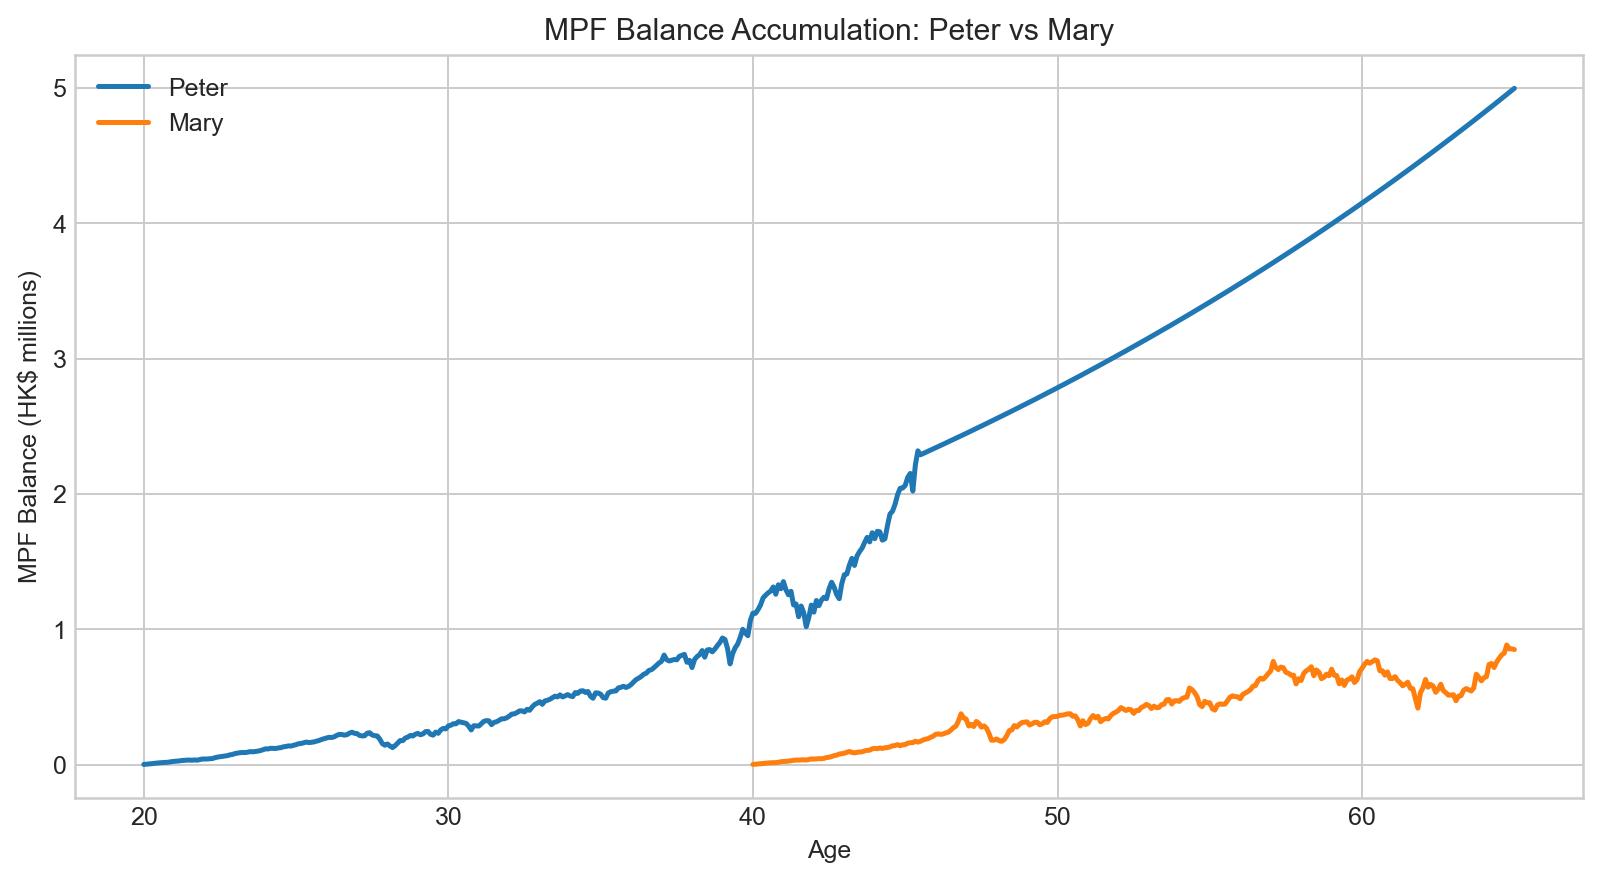
\includegraphics[width=0.92\textwidth]{../output/fig1_balance_over_age.png}
  \caption{MPF balance accumulation: Peter versus Mary}
  \label{fig:balance}
\end{figure}

\subsection*{3. Advantages and Disadvantages}

\textbf{Advantages:}
\begin{enumerate}
  \item \textbf{Clear property rights and portability:} Individual accounts suit Hong Kong's mobile labour market; no employer-credit risk as in DB plans.
  \item \textbf{Employer matching:} The employer's 5\% contribution doubles savings without additional employee cost.
  \item \textbf{Investment choice:} Members can select funds aligned with risk tolerance.
  \item \textbf{Tax incentives:} TVC of up to HK\$60,000 per year is tax-deductible.
  \item \textbf{Compounding:} Early starters benefit enormously from decades of compound growth (the ``Rule of 72'': at 4\% p.a., wealth doubles roughly every 18 years; 45 years yields $\sim$6$\times$ compounding versus $\sim$2.7$\times$ over 25 years).
\end{enumerate}

\textbf{Disadvantages:}
\begin{enumerate}
  \item \textbf{Investment and sequence risk:} Members bear full downside risk; a pre-retirement market crash can sharply erode terminal value.
  \item \textbf{No risk pooling:} Unlike DB plans, there is no cross-subsidy for longevity or investment shortfalls.
  \item \textbf{Low replacement ratio:} Even Peter achieves only 36\% replacement from mandatory contributions, below the 60--70\% commonly recommended.
  \item \textbf{Fee drag and behavioural erosion:} Management fees compound negatively; poor fund switching further reduces net returns.
  \item \textbf{Late starter penalty:} Mary's 9.1\% replacement ratio shows that starting at 40 cannot be fully offset by fund selection.
\end{enumerate}

\subsection*{4. Start Age versus Fund Choice}

Table~\ref{tab:age} reports replacement ratios by start age. Table~\ref{tab:fundswap} reports fund-swap sensitivity at fixed start ages.

\begin{table}[H]
  \centering
  \caption{Replacement ratio by start age and fund}
  \label{tab:age}
  \begin{tabular}{@{}ccrr@{}}
    \toprule
    Start Age & Fund & Final Balance (HK\$) & Replacement Ratio \\
    \midrule
    20 & Global & 4,996,362 & 36.0\% \\
    20 & Hong Kong & 2,427,886 & 17.5\% \\
    30 & Global & 3,417,078 & 30.0\% \\
    30 & Hong Kong & 1,500,213 & 13.2\% \\
    40 & Global & 2,063,587 & 22.1\% \\
    40 & Hong Kong & 850,862 & 9.1\% \\
    50 & Global & 520,922 & 6.9\% \\
    50 & Hong Kong & 457,617 & 6.0\% \\
    \bottomrule
  \end{tabular}
\end{table}

\begin{table}[H]
  \centering
  \caption{Fund-swap sensitivity}
  \label{tab:fundswap}
  \begin{tabular}{@{}lcccc@{}}
    \toprule
    Name & Assigned RR & Swapped RR & Change (pp) \\
    \midrule
    Peter (age 20) & 36.0\% & 17.5\% & $-18.5$ \\
    Mary (age 40) & 9.1\% & 22.1\% & $+13.0$ \\
    \bottomrule
  \end{tabular}
\end{table}

\textbf{Key finding:} Comparing start ages at the same fund shows a \textbf{27 percentage-point gap} (36\% versus 9.1\% for global and Hong Kong funds at ages 20 and 40). Peter at age 20 with the underperforming Hong Kong fund (17.5\%) still ends with a far higher balance than Mary. \textbf{Contribution horizon dominates fund selection} because terminal value is exponentially sensitive to time and only power-sensitive to return.

\begin{figure}[H]
  \centering
  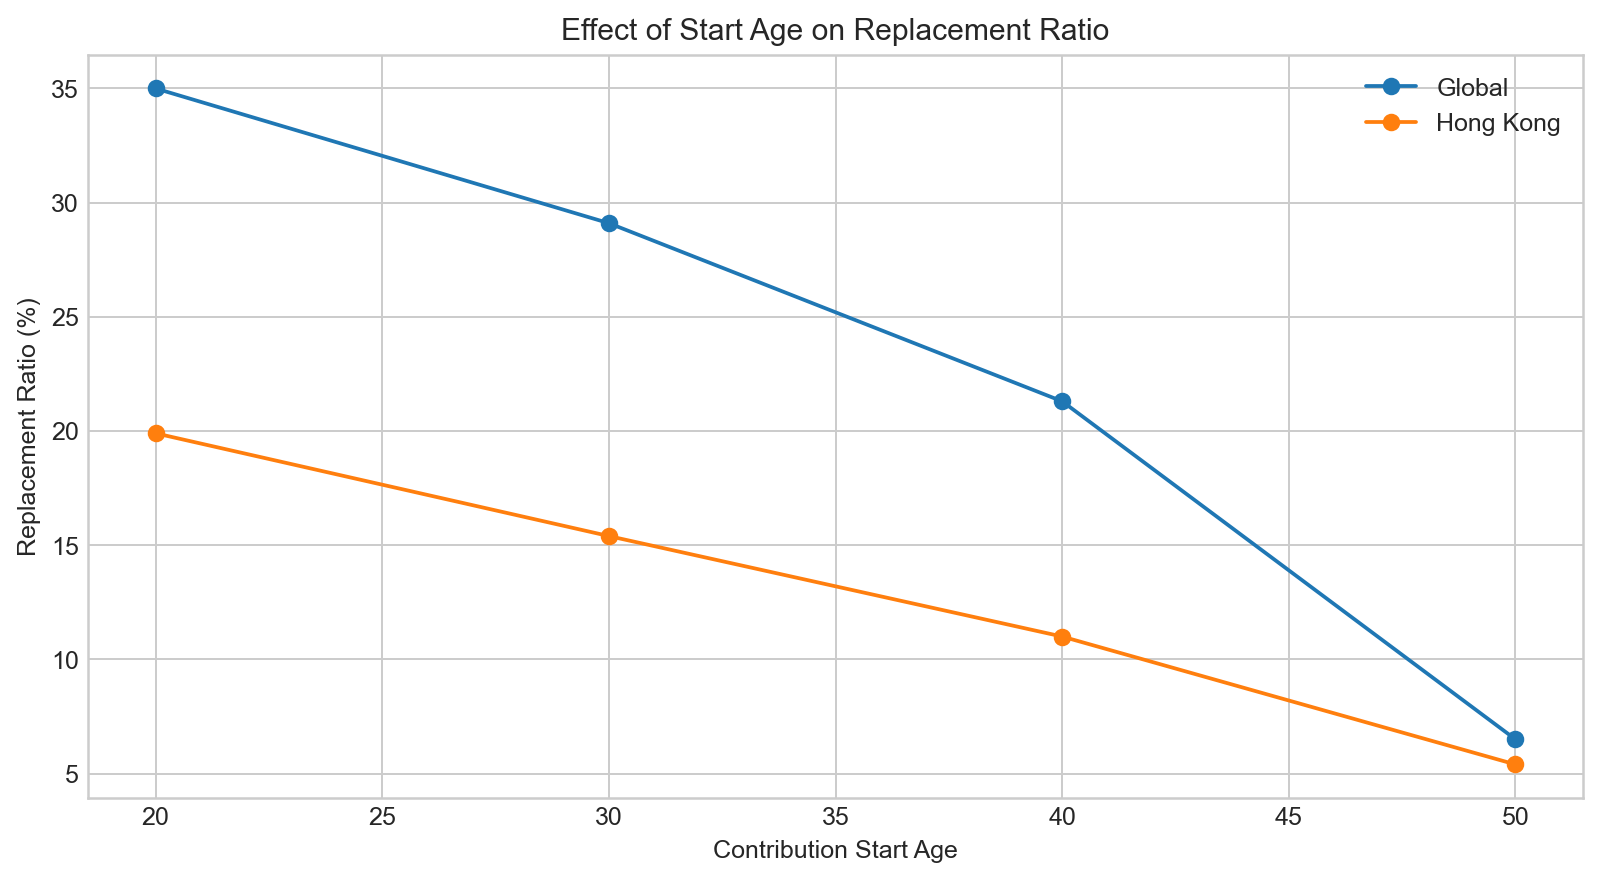
\includegraphics[width=0.92\textwidth]{../output/fig3_start_age_sensitivity.png}
  \caption{Effect of start age on replacement ratio}
  \label{fig:age}
\end{figure}

\subsection*{5. Living Expenses, Inflation, and Extra Contributions}

Financial planners often target a \textbf{60--70\% replacement ratio}. Using final monthly salary from Table~\ref{tab:baseline} ($60\% \times \text{final monthly salary} - \text{MPF monthly income}$): Peter's gap is approximately HK\$11,103; Mary's gap is approximately HK\$15,870.

Salaries and mandatory contributions are indexed to CPI, but real purchasing power of retirement income depends on whether investment returns exceed inflation. A 1\% fee differential over 45 years can materially reduce the final balance (e.g., Peter's balance falls from HK\$4.99M at 1\% fees to about HK\$4.32M at 1.5\% fees in a sensitivity check).

\begin{table}[H]
  \centering
  \caption{TVC required to reach target replacement ratio}
  \label{tab:tvc}
  \begin{tabular}{@{}lcccc@{}}
    \toprule
    Member & Current RR & Target RR & Extra Monthly TVC (HK\$) \\
    \midrule
    Peter & 36.0\% & 60\% & 1,582 \\
    Peter & 36.0\% & 70\% & 2,242 \\
    Mary & 9.1\% & 60\% & 13,205 \\
    Mary & 9.1\% & 70\% & 15,799 \\
    \bottomrule
  \end{tabular}
\end{table}

\begin{figure}[H]
  \centering
  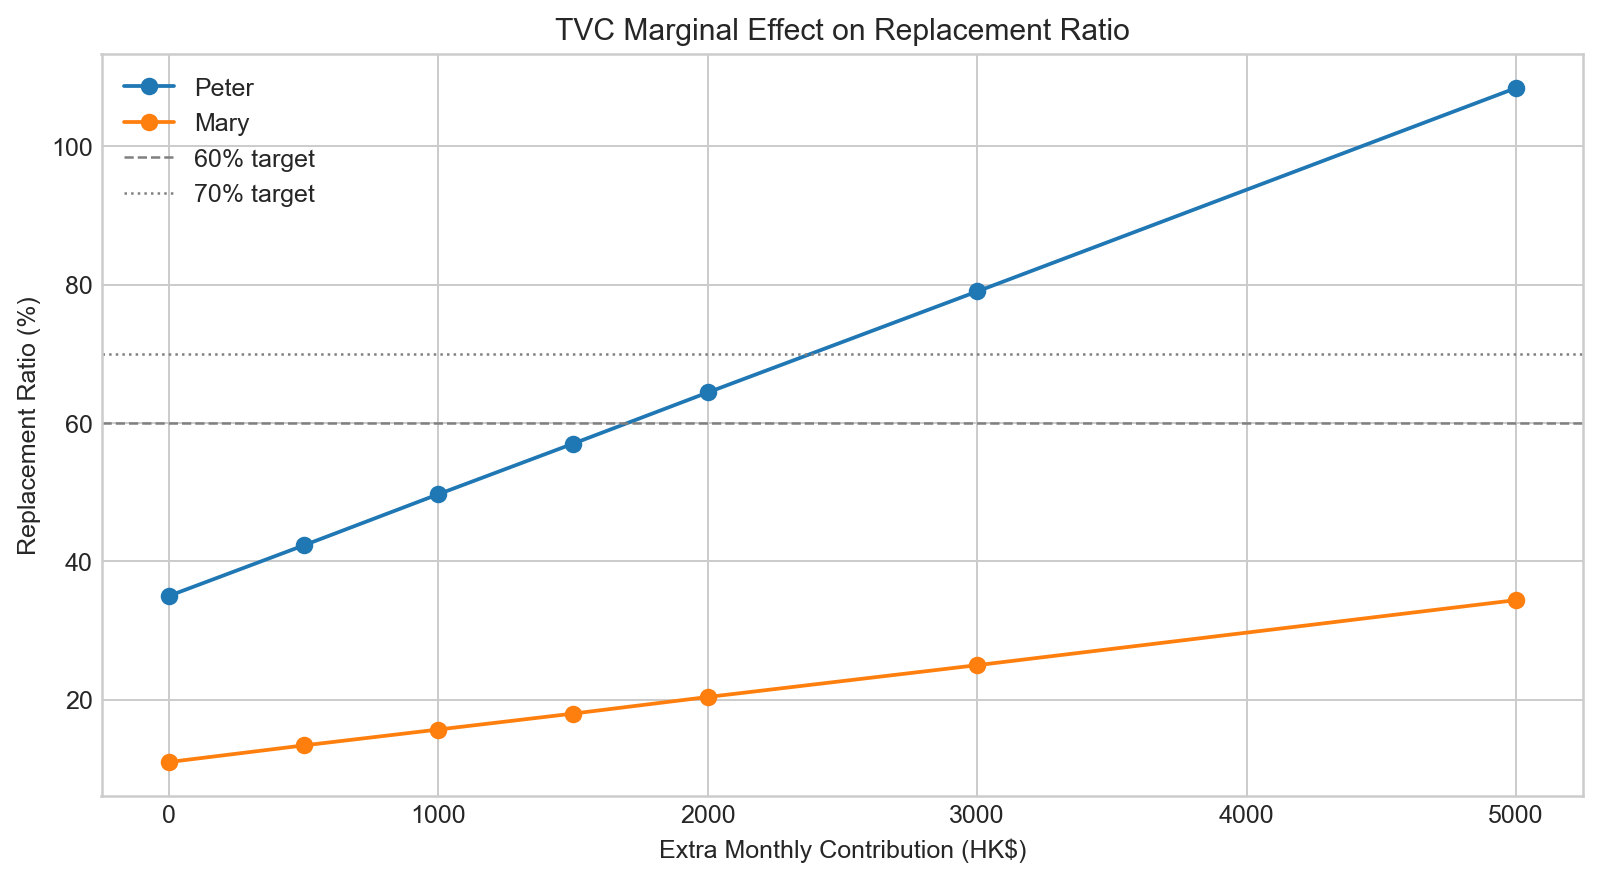
\includegraphics[width=0.92\textwidth]{../output/fig4_tvc_marginal_effect.png}
  \caption{Marginal effect of TVC on replacement ratio}
  \label{fig:tvc}
\end{figure}

Mary urgently needs substantial TVC or other income sources. Peter still requires about HK\$1,600 per month extra to reach 60\% replacement, achievable within the TVC tax-deductible limit (HK\$60,000/year $\approx$ HK\$5,000/month). By contrast, Mary's required TVC of HK\$13,205/month far exceeds the TVC cap; only the first HK\$5,000/month enjoys tax relief---the remainder must come from non-deductible VC or third-pillar savings.

\section*{(c) Supporting Retirement Under DC with the Social Security System}

\subsection*{1. Hong Kong Three-Pillar Framework}

Unlike Canada's CPP or US Social Security, Hong Kong has \textbf{no universal earnings-related public pension}. Government support is means-tested and \textbf{layered}:
\begin{itemize}
  \item \textbf{First pillar} provides a floor for low-asset, low-income seniors (CSSA strictest; OALA asset/income-tested; OAA more universal but smaller)
  \item \textbf{Second pillar} (MPF) is the mandatory base for all employed persons
  \item \textbf{Third pillar} is the main lever for maintaining pre-retirement living standards
\end{itemize}

For middle-income workers such as Peter and Mary, first-pillar benefits are largely \textbf{unavailable} when MPF balances are counted in asset tests---retirement income must come from MPF plus voluntary savings, not from simple ``stacking'' of pillars.

\subsection*{2. Old Age Living Allowance (OALA)}

Eligible Hong Kong residents aged 65+ may receive Normal OALA (HK\$2,065/month) or Higher OALA (HK\$4,185/month) in 2025/26, subject to income and asset tests. For a single person, the asset limit for both tiers is approximately HK\$401,000. \textbf{MPF accrued benefits not yet withdrawn are counted as assets}. This creates a \textbf{crowding-out effect}: the more DC wealth a member accumulates, the less likely they qualify for first-pillar support---the two are not simply additive.

\subsection*{3. Combined Retirement Income}

Table~\ref{tab:income} reports \textbf{actual} eligibility. Peter (MPF balance HK\$4.99M) and Mary (HK\$851K) both exceed the asset limit and therefore receive \textbf{no OALA} when MPF is counted. Table~\ref{tab:income_hyp} shows hypothetical amounts \emph{only if} assets were below the limit (illustrative contrast).

\begin{table}[H]
  \centering
  \caption{Retirement income after OALA asset test (MPF counted)}
  \label{tab:income}
  \small
  \begin{tabular}{@{}l r r r r r@{}}
    \toprule
    Member & MPF Balance & Asset Limit & MPF Income & OALA & Combined RR \\
    \midrule
    Peter & 4,996,362 & 401,000 & 16,655 & 0 & 36.0\% \\
    Mary & 850,862 & 401,000 & 2,836 & 0 & 9.1\% \\
    \bottomrule
  \end{tabular}
\end{table}

\begin{table}[H]
  \centering
  \caption{Hypothetical OALA (if MPF not counted---not applicable to Case III)}
  \label{tab:income_hyp}
  \small
  \begin{tabular}{@{}l l r r r r@{}}
    \toprule
    Member & Scenario & MPF & OALA & Total & Combined RR \\
    \midrule
    Peter & Normal OALA & 16,655 & 2,065 & 18,720 & 40.5\% \\
    Peter & Higher OALA & 16,655 & 4,185 & 20,840 & 45.0\% \\
    Mary & Normal OALA & 2,836 & 2,065 & 4,901 & 15.7\% \\
    Mary & Higher OALA & 2,836 & 4,185 & 7,021 & 22.5\% \\
    \bottomrule
  \end{tabular}
\end{table}

\begin{figure}[H]
  \centering
  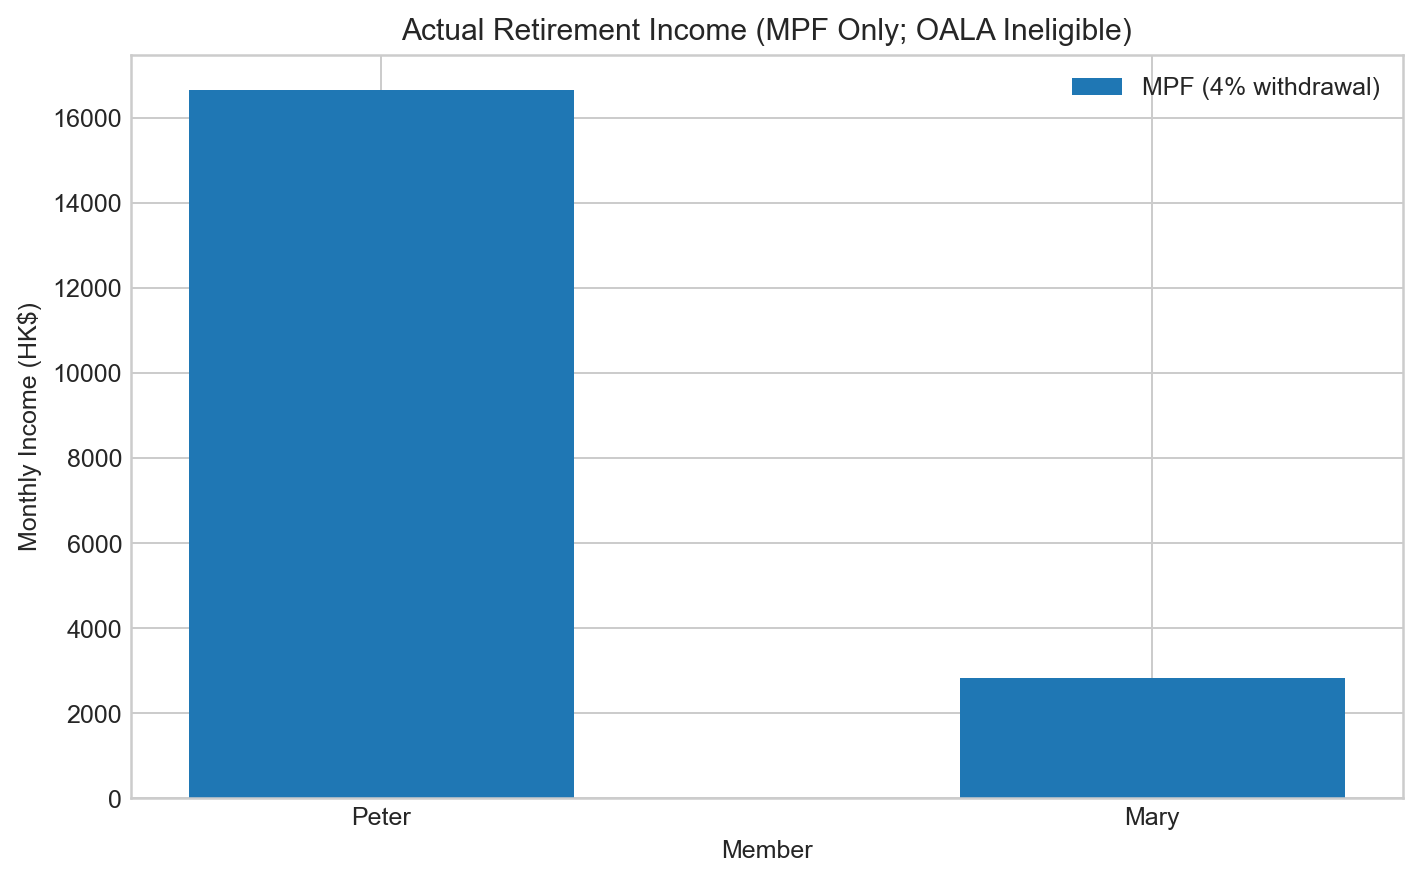
\includegraphics[width=0.78\textwidth]{../output/fig2_income_breakdown.png}
  \caption{Actual retirement income (MPF only; OALA ineligible under asset test)}
  \label{fig:income}
\end{figure}

\subsection*{4. Illustrative Strategies}

\textbf{Peter (retirement 2045):}
\begin{itemize}
  \item MPF provides a solid base (36\% replacement ratio) but OALA is \textbf{ineligible} given expected MPF assets.
  \item Add TVC of about HK\$1,600 per month to reach 60\% replacement from MPF alone (within the TVC tax cap).
  \item Adopt a \textbf{lifecycle glide path}: high equity allocation when young, gradually shifting to bonds/capital-preservation funds after age 55 to mitigate sequence risk---rather than holding 100\% global equity for 45 years.
  \item Annuitise part of the MPF balance to create a guaranteed lifetime income floor against longevity risk.
\end{itemize}

\textbf{Mary (retirement 2025):}
\begin{itemize}
  \item Mandatory MPF alone is severely inadequate (9.1\% replacement ratio); OALA is \textbf{ineligible} (balance HK\$851K $>$ HK\$401K limit).
  \item Delaying retirement to age 70 raises the replacement ratio only modestly (to 10.9\% in our simulation)---extra years of contribution help, but cannot offset 20 years of lost compounding.
  \item Required extra savings far exceed the TVC tax cap; combine non-deductible VC, third-pillar savings, and possible part-time work.
  \item Annuitisation and delayed withdrawal can still improve income security given limited account size.
\end{itemize}

A realistic plan for Mary---MPF (HK\$2,836) plus third-pillar savings or part-time income (e.g., HK\$5,000/month)---yields about HK\$7,836 per month, still below the 60\% target of HK\$18,706. Even the hypothetical Higher OALA scenario (Table~\ref{tab:income_hyp}) reaches only 22.5\%.

\begin{table}[H]
  \centering
  \caption{Mary: delayed retirement sensitivity}
  \label{tab:delay}
  \begin{tabular}{@{}lrrr@{}}
    \toprule
    Retirement Age & Contribution Years & MPF Balance (HK\$) & Replacement Ratio \\
    \midrule
    65 & 25.1 & 850,862 & 9.1\% \\
    67 & 27.1 & 930,635 & 9.6\% \\
    70 & 30.1 & 1,128,770 & 10.9\% \\
    \bottomrule
  \end{tabular}
\end{table}

\subsection*{5. Conclusions on Extra Contributions}

\begin{table}[H]
  \centering
  \caption{Summary recommendations}
  \label{tab:conclusion}
  \begin{tabular}{@{}lcc@{}}
    \toprule
    Question & Peter & Mary \\
    \midrule
    Is mandatory MPF sufficient? & No (36\%) & No (9.1\%) \\
    Should they add TVC? & Yes, moderate & Yes, urgent \\
    Can social security fill the gap? & No (asset test) & No (asset test) \\
    \bottomrule
  \end{tabular}
\end{table}

Hong Kong's DC system shifts retirement responsibility to the individual. Early, consistent contributions---as in Peter's case---are the most powerful lever. Social security (OALA) provides a safety net for \textbf{low-asset} retirees but is crowded out by MPF accumulation for the middle class. \textbf{Both Peter and Mary should make extra contributions; the urgency and required amount are far greater for Mary.}

\subsection*{6. Core Conclusions}

\begin{enumerate}
  \item Mandatory MPF alone cannot maintain pre-retirement living standards; voluntary savings are essential.
  \item \textbf{Contribution start date} is the dominant determinant of DC outcomes---time compounding outweighs fund selection.
  \item Hong Kong's first pillar provides a floor, not a supplement, for middle-income members with meaningful MPF balances.
  \item A complete retirement plan combines mandatory MPF, voluntary contributions (TVC within tax limits), third-pillar savings, lifecycle de-risking, and partial annuitisation.
\end{enumerate}

\section*{Key Formulae}

Future value with CPI-linked contributions (monthly simulation):
\begin{equation}
  FV = \sum_{t=1}^{n} PMT_0 (1+g)^{t-1} \prod_{k=t+1}^{n}(1+r_k)
\end{equation}
where $PMT_0$ is the initial monthly contribution, $g$ is the annual contribution growth rate (CPI), $r_k$ is the net return in period $k$, and $n$ is the number of contribution periods.

When $r$ and $g$ are constant and $r \neq g$, the growing-annuity closed form is:
\begin{equation}
  FV = PMT_0 (1+r) \cdot \frac{(1+r)^n - (1+g)^n}{r - g}
\end{equation}

Replacement ratio with a 4\% withdrawal rate:
\begin{equation}
  RR = \frac{FV \times 0.04}{Salary_{final}}
\end{equation}

Required monthly TVC to reach target replacement ratio $\rho^*$: solve for $PMT_{TVC}$ such that
\begin{equation}
  \rho^* = \frac{0.04 \times FV(PMT_0, g, r, n) + 0.04 \times FV(PMT_{TVC}, g, r, n')}{Salary_{final}}
\end{equation}
where $n'$ is the number of periods over which extra contributions are made (here, the full contribution horizon). Table~\ref{tab:tvc} values are obtained by binary search on this condition in the simulation model.

Monthly income gap to a 60\% target:
\begin{equation}
  Gap_{monthly} = 0.60 \times \frac{Salary_{final}}{12} - \frac{FV_{MPF} \times 0.04}{12}
\end{equation}

\begin{thebibliography}{9}
  \bibitem{mpfa} Mandatory Provident Fund Schemes Authority, \textit{MPF Fund Performance Platform}, \url{https://mfp.mpfa.org.hk/}.
  \bibitem{swd} Social Welfare Department, \textit{Old Age Living Allowance}, \url{https://www.swd.gov.hk/oala/}.
  \bibitem{csd} Census and Statistics Department, \textit{Composite Consumer Price Index}.
  \bibitem{ira} Investopedia, \textit{Individual Retirement Account (IRA)}, \url{https://www.investopedia.com/terms/i/ira.asp}.
\end{thebibliography}

\appendix
\section*{Appendix: Simulation Reproducibility}

All numerical results are generated by the Python pipeline in \texttt{case3/}. To reproduce tables and figures:
\begin{verbatim}
cd case3
python3 main.py
python3 src/validate.py
\end{verbatim}

Output files are stored in \texttt{case3/output/}. Assumptions are documented in \texttt{case3/data/assumptions.md}.

\end{document}
